\subsection{Rotational action spectroscopy}
\label{subsec:action:methods:rotational}

Action spectroscopy for measuring rotational transitions is very challenging
since the rotational transition energies are much lower than vibrational or
electronic states (see Table \ref{tab:electromagnetic_spectrum}). While
vibrational and electronic action spectroscopic methods have been available for
trapped ions and ionic clusters since the 1980s, the first rotational action
spectroscopic methods appeared only a decade ago from Schlemmer's group
\cite{Asvany2008}.

This section provides a brief summary of the detailed review by
\citet{Asvany2021} but focuses only on rotational action spectroscopic methods.
Figure \ref{fig:action:methods:rotational} shows the summary of rotational
action spectroscopic methods schematic diagrams.

\subsubsection{Rotational LIR}
\label{subsec:rotational-LIR}

Schlemmer and coworkers showed the first realization of pure rotational action
spectroscopy in a cryogenic trap using a direct-LIR method (as discussed in
Section \ref{subsec:action:methods:vibrational:LIR}) \cite{Asvany2008}. Using
this approach, they measured the lowest-lying rotational transitions
\emph{para-}H$_2$D$^+$ and \emph{ortho-}D$_2$H$^+$, two astronomically
important molecular ions that exhibit large rotational energy spacing (1.37 THz
and 1.48 THz for the ground state transitions, respectively). The on-resonance
laser-induced reactions of H$_2$D$^+$ and D$_2$H$^+$ held in a cold ion trap
increases the reactivity (producing H$_3^+$ and H$_2$D$^+$, respectively) with
a neutral H$_2$ reaction partner. Therefore the rotational transitions of the
investigated ions are reflected in the yield of the reaction products as shown
in Figure \ref{fig:action:methods:rotational:LIR}.

\subsubsection{Double resonance methods}
\label{subsec:action:methods:rotational:DR}

As discussed in Section \ref{subsec:action:methods:vibrational:LIICG} there are
limitations to the direct-LIR technique. Therefore further rotational action
spectroscopic techniques were later developed to generalise the scheme for a
wide range of molecular ions, such as using a double resonance approach. A
vibrational action spectroscopy scheme can be used to perform high-resolution
rotational spectroscopy by double resonance. In other words, if a molecule has
a vibrational action spectroscopy scheme with a rotational resolution, the
spectroscopy can easily be extended into the rotational domain by a double
resonance approach; the possibilities are as follows:

\textbf{\emph{via} LIR}: As shown in Figure \ref{fig:action:methods:rotational:DR_LIR}, this method uses a combination of infrared (IR) and Terahertz (THz) radiation to irradiate ions. The frequency of the IR photon is kept fixed on a rovibrational transition. The signal is monitored by counting the number of the product ions produced as a function of the THz frequency \cite{Gartner2013,jusko_two-photon_2014}. The signal can be depletion or gain depending on whether the IR is fixed at a rotational ground or excited state.

\textbf{\emph{via} predissociation:} Predissociation is another effective vibrational action spectroscopic technique (see Section \ref{subsec:action:methods:vibrational:IRPD}). Based on prior IR predissociation work by Dopfer and collaborators \cite{olkhov_intermolecular_1999}, the vibrational-rotational predissociation via double resonance approach (see Figure \ref{fig:action:methods:rotational:DR_THz_IR}) has been shown for the first time for the He$-$CH$_3^+$ complex \cite{Topfer2018}.

\textbf{\emph{via} electron detachment:}
This high-resolution rotational action spectroscopy via double resonance schemes method is suitable for molecular anions. Wester and coworkers \cite{lee_terahertz-visible_2016} devised an action scheme using state-selective electron photodetachment via fixed \qt{visible} (vis) frequency radiation (see Figure \ref{fig:action:methods:rotational:DR_THz_Vis}), and demonstrated it by measuring the two lowest rotational transitions of OD$^-$. The molecular anion counts are monitored as a function of frequency (rotational photon). On rotational resonance, the radiation populates the initial state probed by a fixed-vis laser which subsequently increases the electron photo-detachment, thereby decreasing molecular ion counts (depletion signal).

\textbf{\emph{via} LIICG: } In LIICG, excitation of the bare cation can inhibit He-attachment in a ternary collision process at 4 K (see Section \ref{subsec:action:methods:vibrational:LIICG}), and this is utilised in this method. The IR laser is fixed at a rovibrational transition; the He-cation molecular ion complexes are monitored as a function of THz frequency (see Figure \ref{fig:action:methods:rotational:DR_THz_IR_LIICG}). The depletion in complex counts on the rotational transition resonance frequency of the bare cation is the signal. It has been demonstrated for protonated methenamine, CH$_2$NH$_2^+$ \cite{Markus2019}.

\subsubsection{ROSAA}
\label{subsec:action:methods:rotational:ROSAA}

The rotational high-resolution rotational action spectroscopy technique
employed in this thesis is ROSAA which is an abbreviation of to
\textbf{RO}tational \textbf{S}tate-dependent \textbf{A}ttachment of rare gas
\textbf{A}toms. This method exploits that the ternary attachment of neutral
atoms (typically He) depends on their rotational quantum state since the
ternary attachment of He is only hindered (or changed, see
Figure\ref{fig:action:methods:rotational:ROSAA}) instead of inhibited as
discussed in LIICG (see Section \ref{subsec:action:methods:vibrational:LIICG}).
\citet{brunken_laboratory_2014} demonstrated it by measuring four pure
high-resolution rotational transitions for C$_3$H$^+$ ($^2\Sigma$).

The fact that helium atoms can theoretically be attached to any cation at low
temperatures ($<15$ K) is a significant advantage of this approach. Several
molecular cations have been studied in the laboratory for the first time with
the state-dependent He attachment approach. High-resolution pure rotational
transition frequencies have been measured using this technique for l-C$_3$H$^+$
\cite{brunken_laboratory_2014}, CF$^+$ \cite{stoffels_laboratory_2016},
SiH$^+$\cite{domenech2017}, HCO$^+$ \cite{salomon_double_2019},
CD$^+$\cite{Brunken2017}, CH$^+$ and $^{13}$CH$^+$\cite{domenech_first_2018},
NH$_3$D$^+$\cite{stoffels_laboratory_2016, domenech_accurate_2018},
NH$_2$D$_2^+$ and NHD$_3^+$ \cite{domenech_accurate_2018},
CN$^+$\cite{thorwirth_pure_2019}, CH$_2$NH$_2^+$\cite{Markus2019},
CH$_3$NH$_3^+$\cite{schmid_rotational_2022}, NO$^+$
\cite{asvany_fundamental_2021}, CCl$^+$\cite{asvany_pure_2021} and CO$^+$ with
resolved Zeeman components from earth magnetic field
\cite{marimuthu_zeeman_2022, Brunken2017} (see Chapter \ref{chapter:CO+}).\\

As mentioned above, the ROSAA technique is employed in this thesis for
characterising the rotational transition of molecular cations. More detail and
in-depth analysis of ROSAA action spectroscopic schemes are explored using
numerical simulations (Section \ref{subsec:ROSAA} and
\ref{subsec:ROSAA-simulation}) for CD$^+$ (see Section
\ref{subsec:rate-constants-laserOn} and \ref{subsec:CD+-kinetics-simulation} )
and CO$^+$ (see Chapter \ref{chapter:CO+}) ions.

\begin{figure}[!htb]
    \centering
    % \begin{adjustbox}{minipage=\linewidth,scale=0.7}
    \Subfigure[0.3]{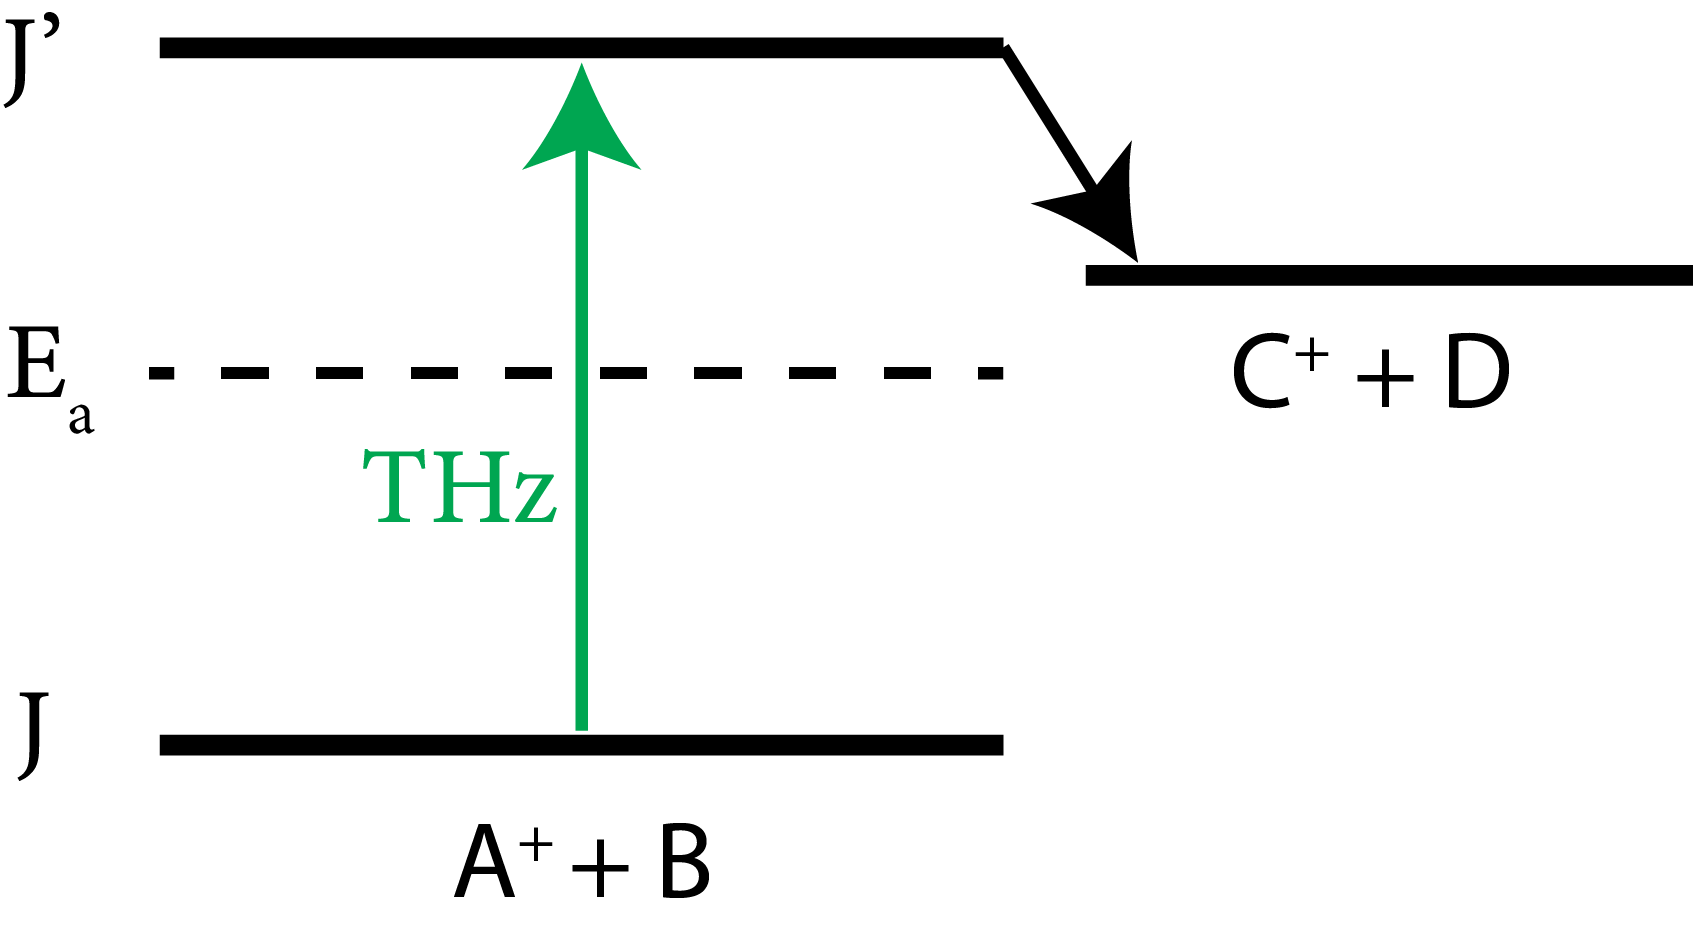
\includegraphics[width=1\textwidth]{figures/intro/rotational-action/LIR.png}}{LIR}{\label{fig:action:methods:rotational:LIR}}
    \hfill
    \Subfigure[0.3]{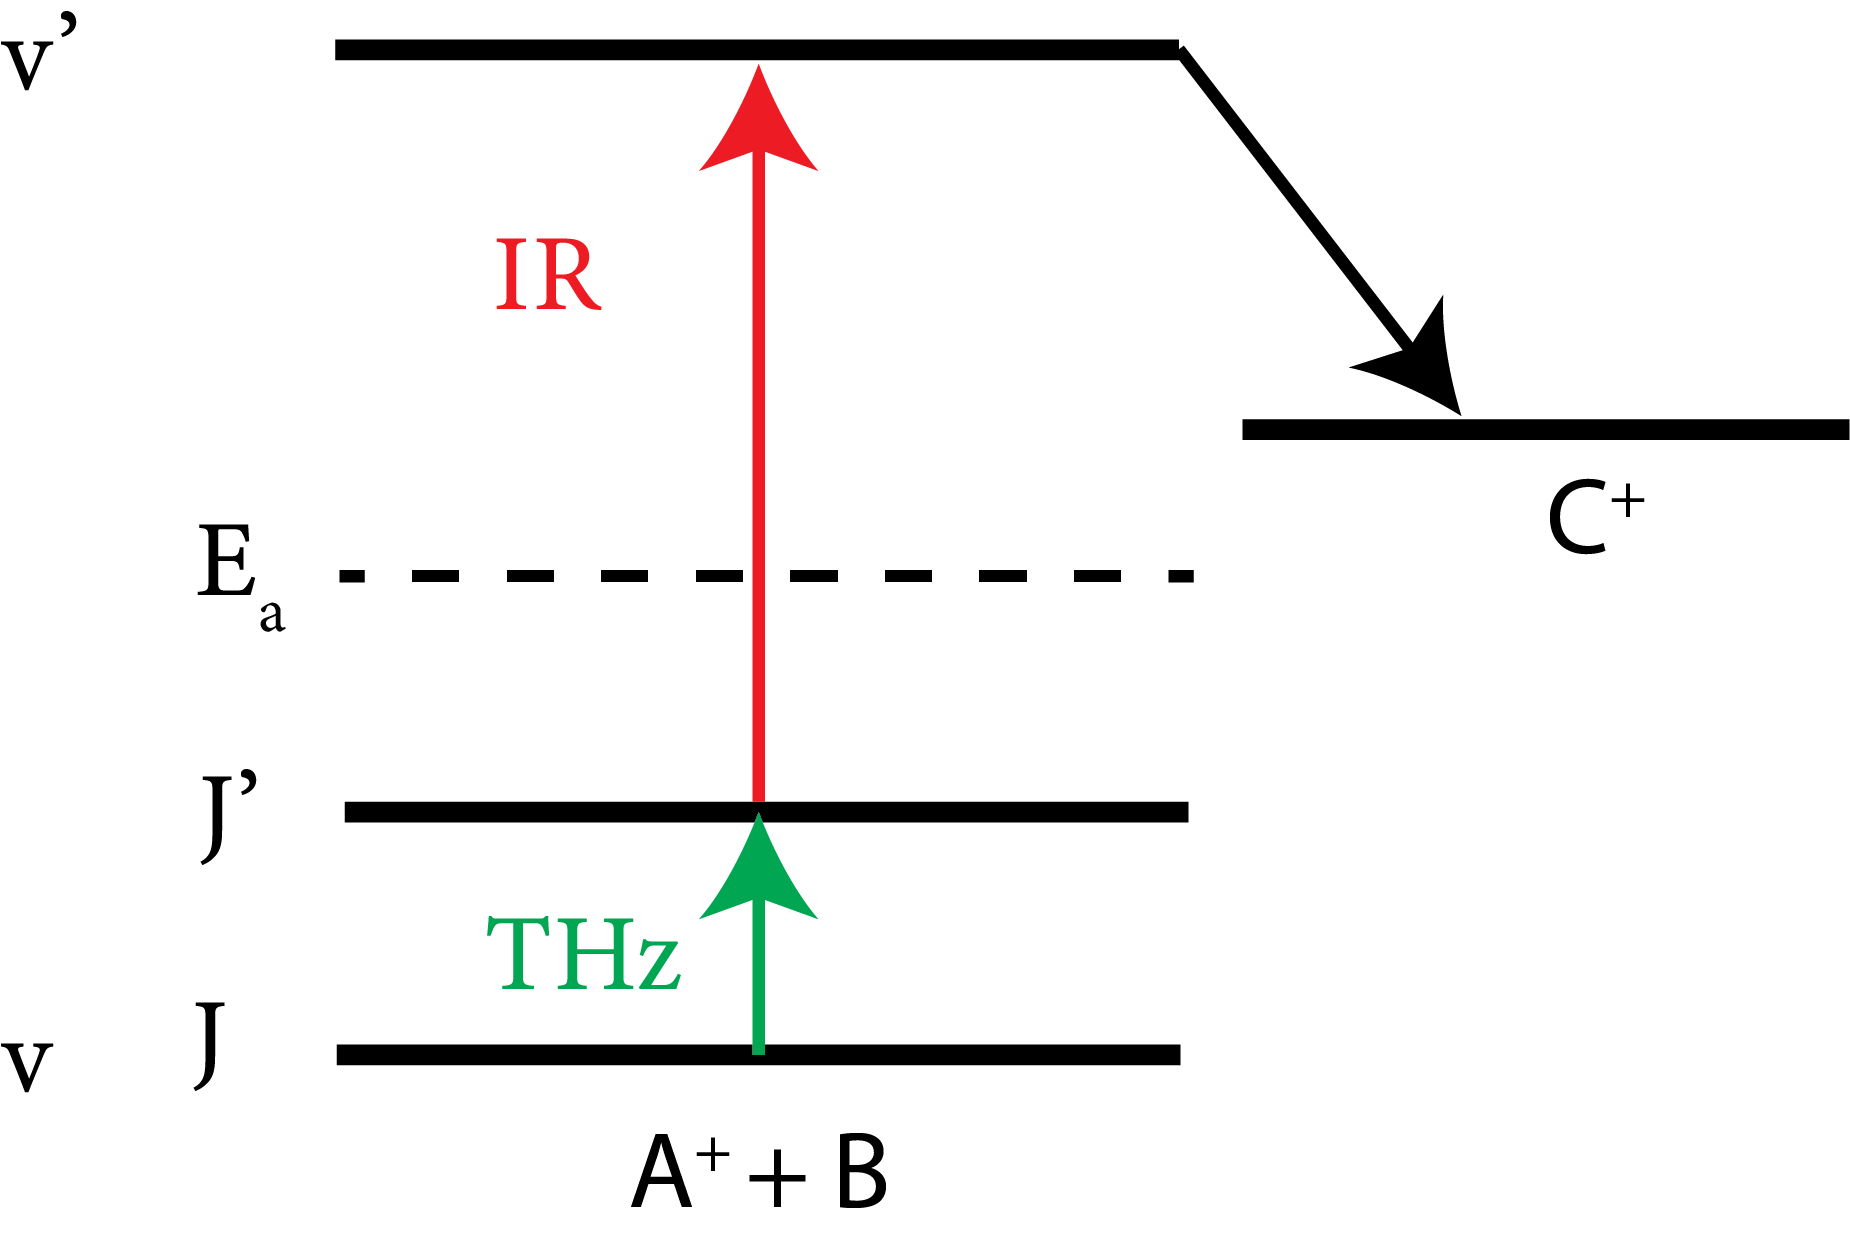
\includegraphics[width=1\textwidth]{figures/intro/rotational-action/DR_LIR.png}}{DR \emph{via} LIR}{\label{fig:action:methods:rotational:DR_LIR}}
    \hfill
    \Subfigure[0.3]{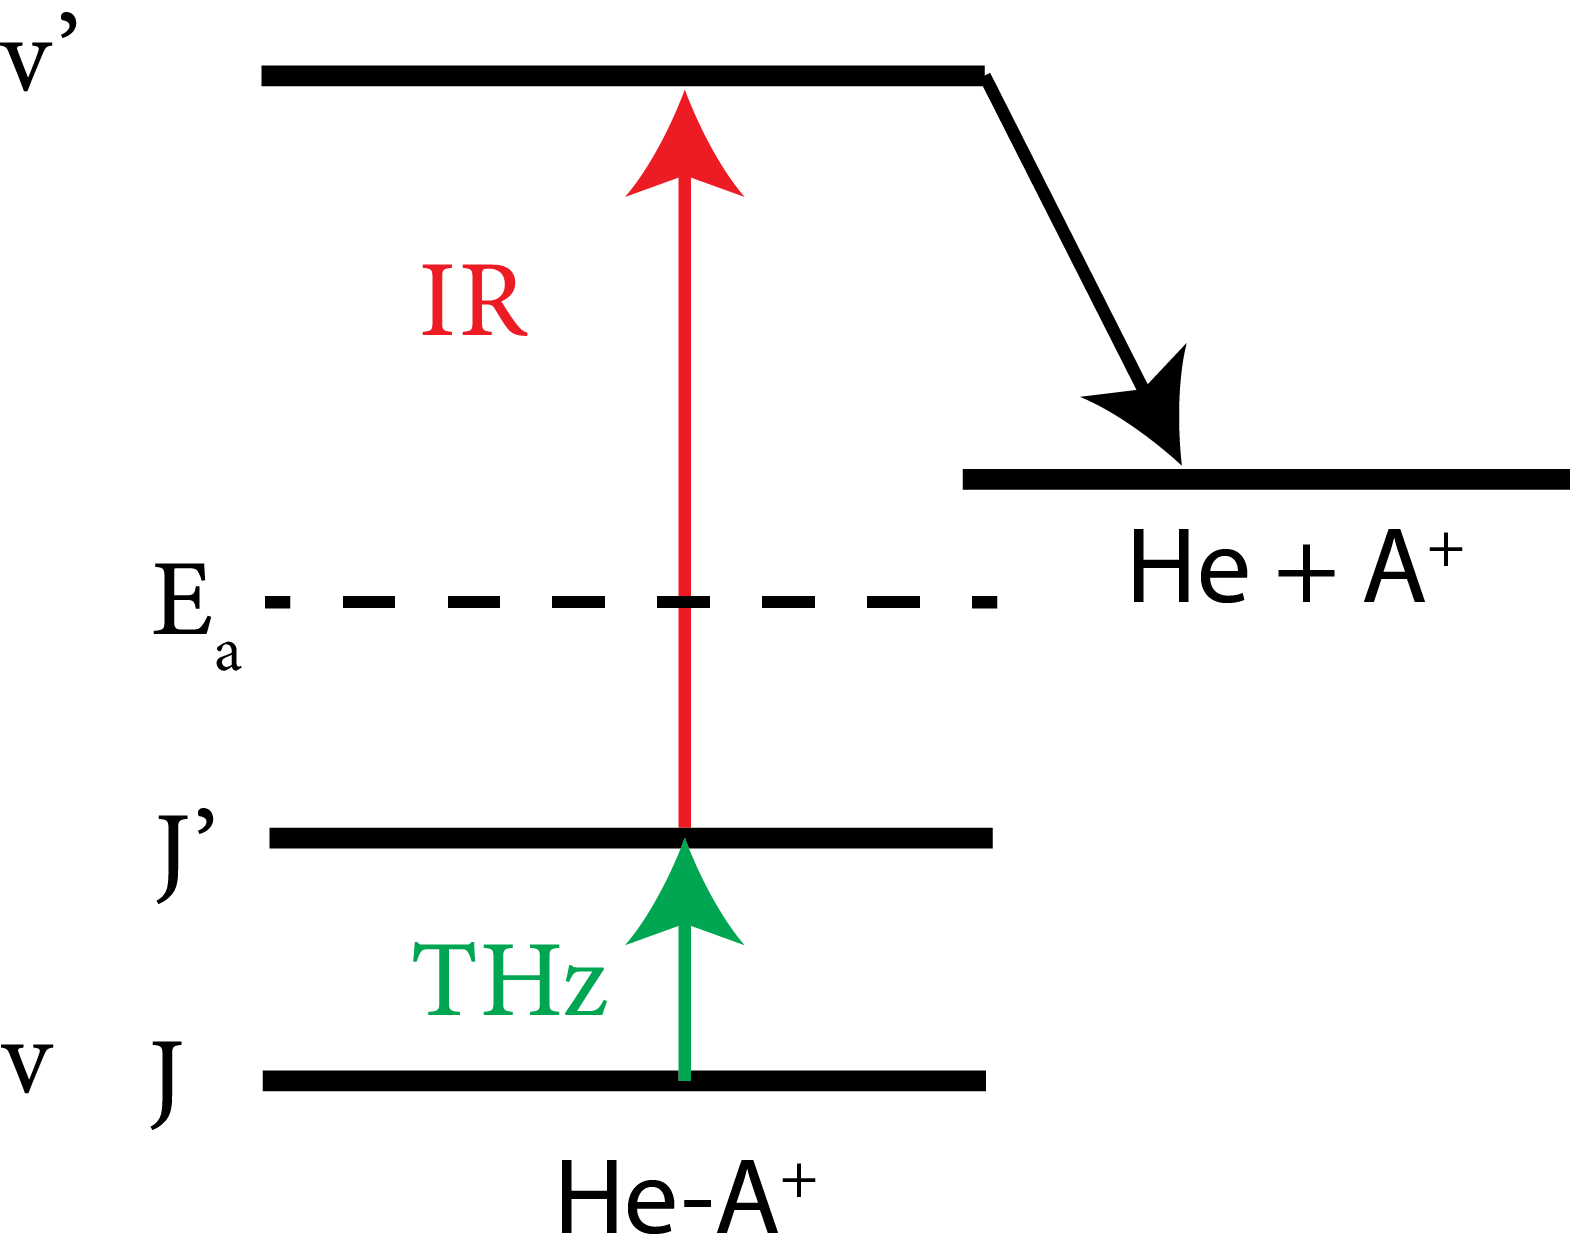
\includegraphics[width=1\textwidth]{figures/intro/rotational-action/DR_THz-IRPD.png}}{DR \emph{via} predis.}{\label{fig:action:methods:rotational:DR_THz_IR}}
    \hfill
    
    \hfill
    
    \Subfigure[0.3]{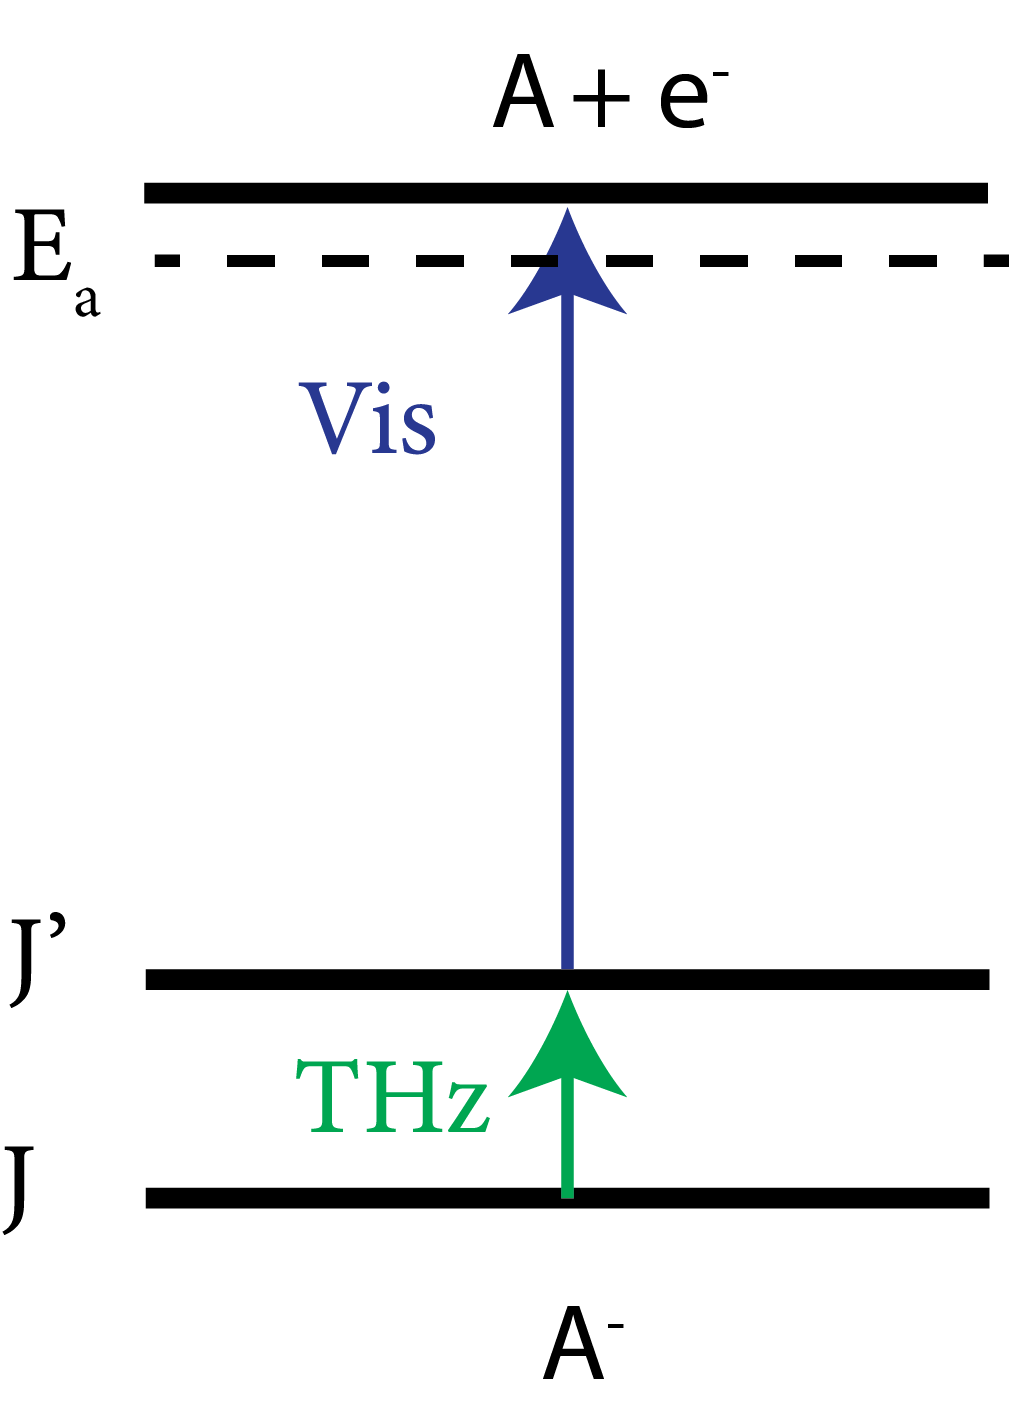
\includegraphics[scale=0.3]{figures/intro/rotational-action/EA.png}}{DR \emph{via} \emph{e}$^-$ det.}{\label{fig:action:methods:rotational:DR_THz_Vis}}
    \hfill
    \Subfigure[0.3]{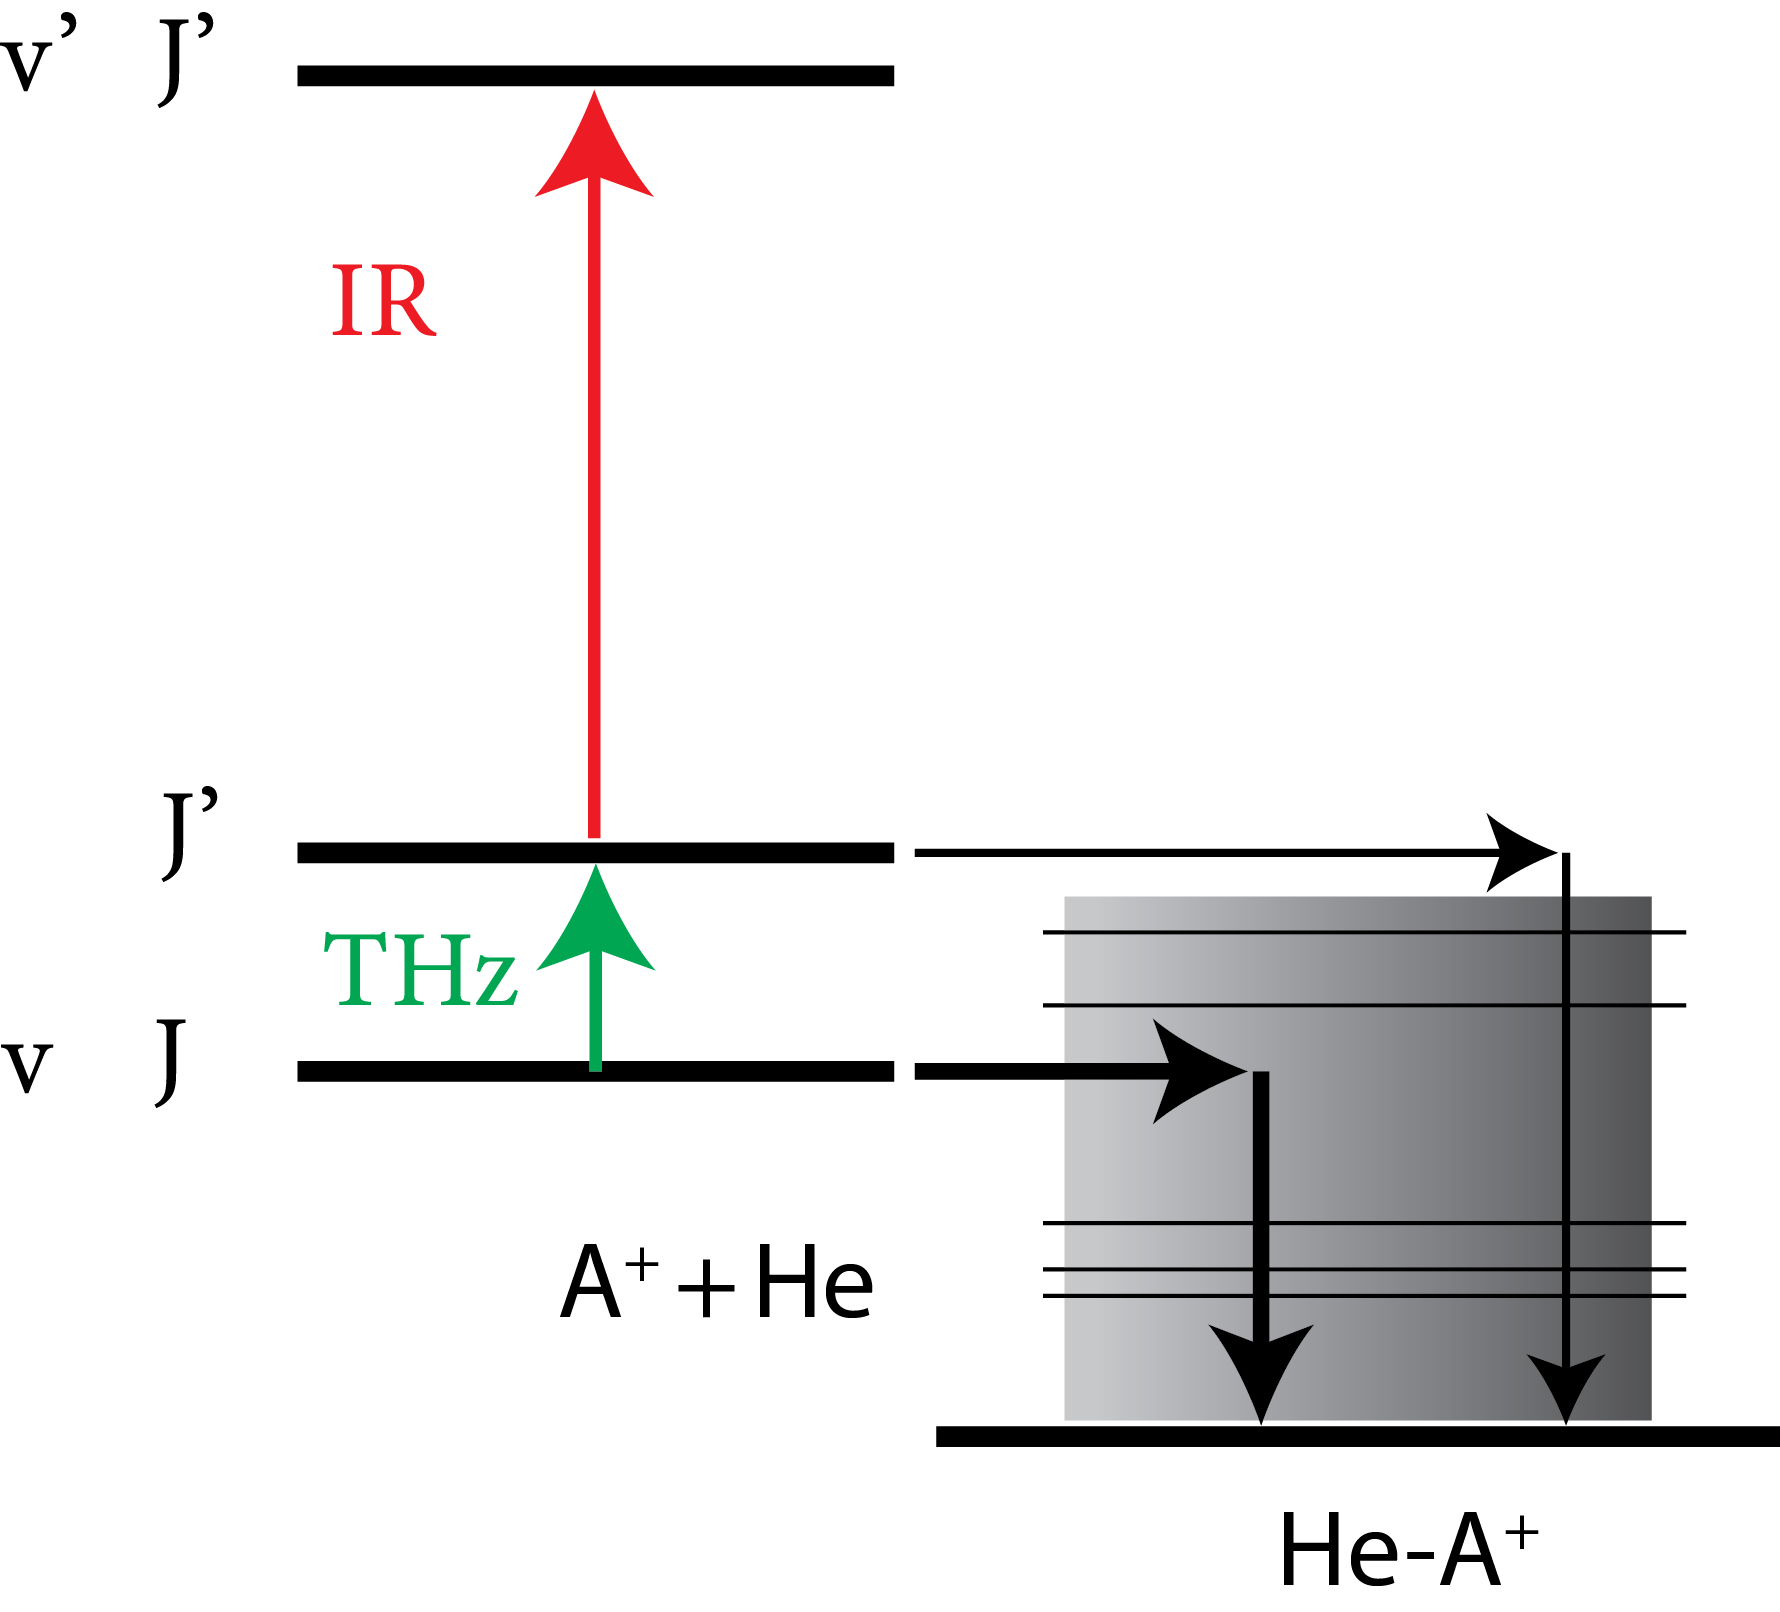
\includegraphics[width=1\textwidth]{figures/intro/rotational-action/DR_THz_IR_LIICG.png}}{DR \emph{via} LIICG}{\label{fig:action:methods:rotational:DR_THz_IR_LIICG}}
    \hfill
    \Subfigure[0.3]{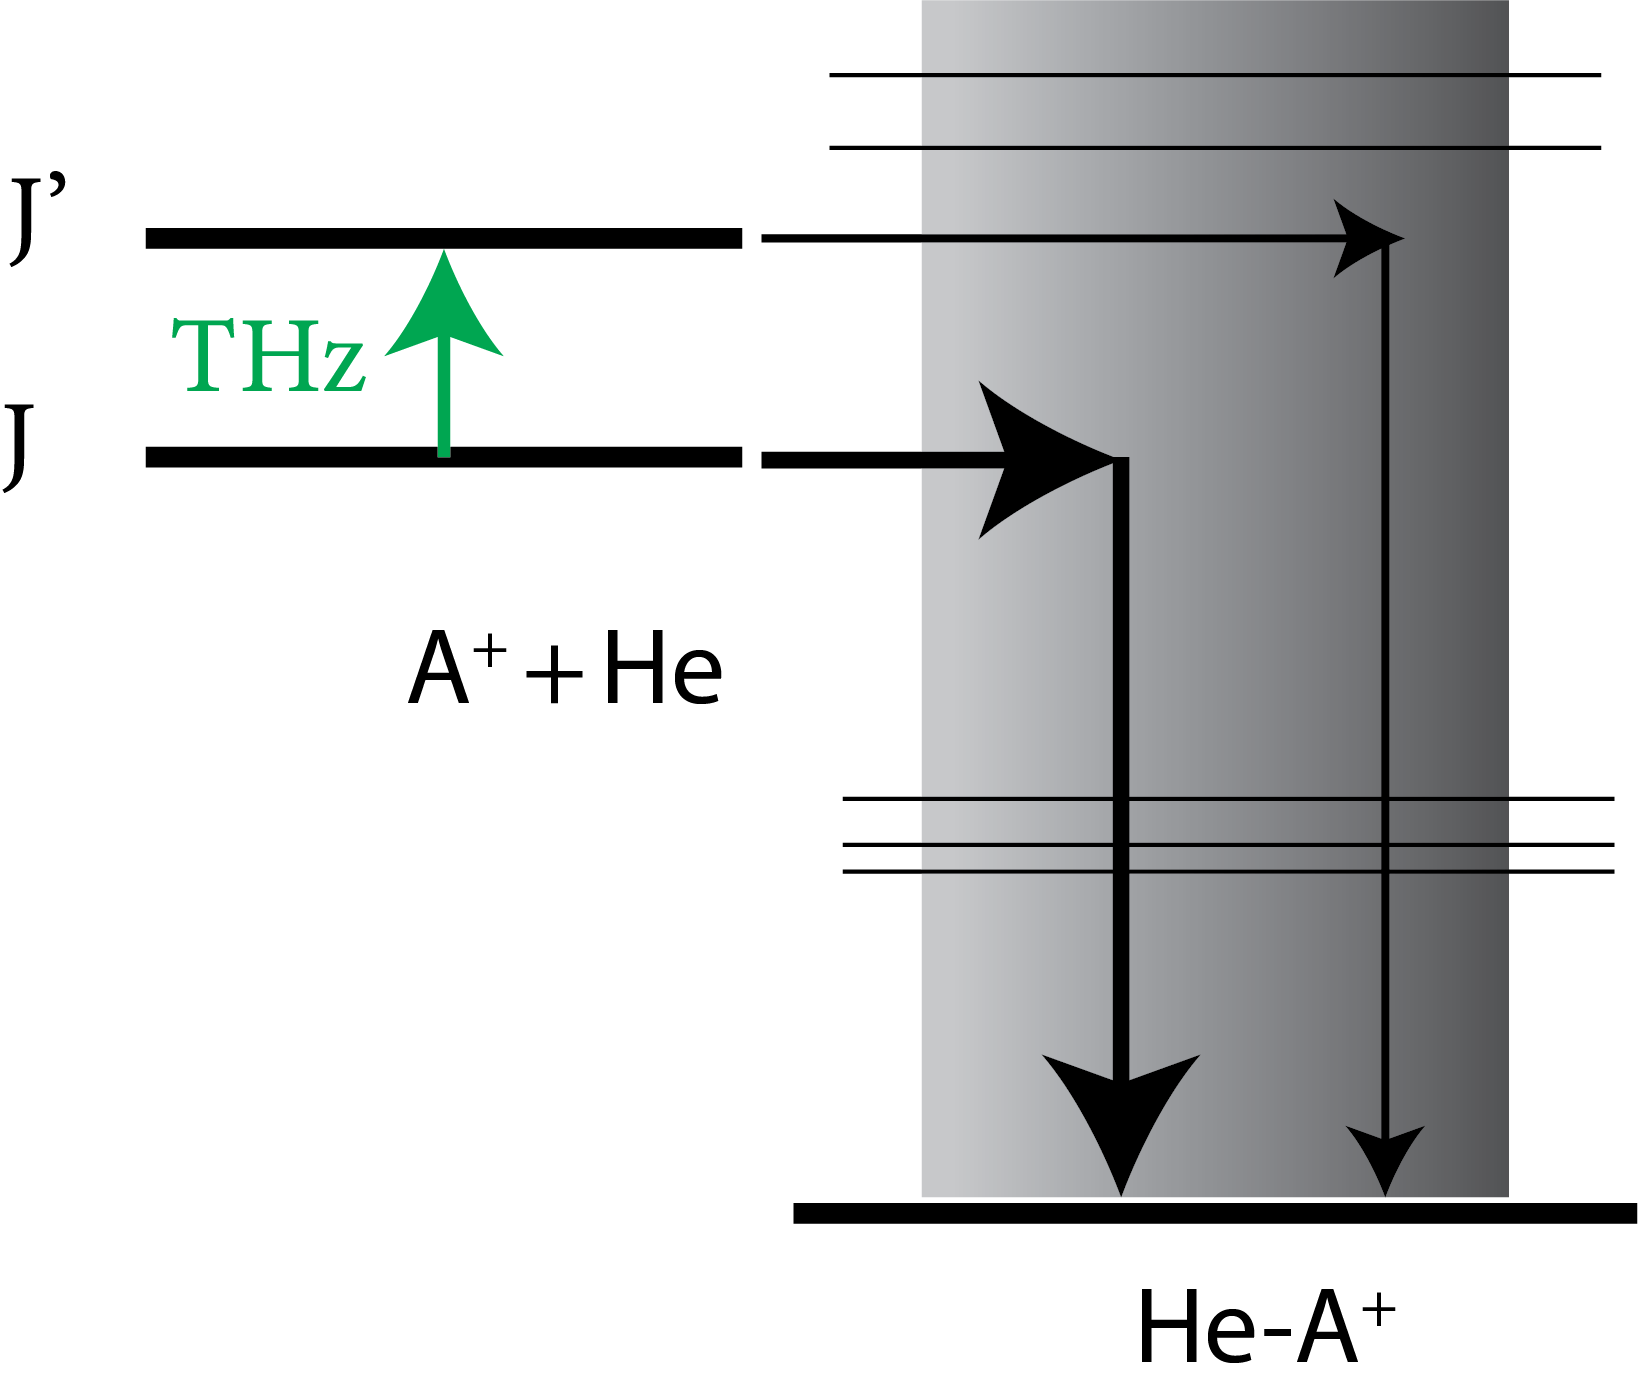
\includegraphics[width=1\textwidth]{figures/intro/rotational-action/ROSAA.png}}{ROSAA}{\label{fig:action:methods:rotational:ROSAA}}
    % \hfill
    % \end{adjustbox}
    \caption{Schematic diagrams of rotational action spectroscopic methods. The captions indicate the corresponding name of the method. DR stands for double resonance. \qt{predis.} and \qt{det.} in (c) and (d) correspond to \qt{predissociation} and \qt{detachment}, respectively. The symbol A and B indicates molecular species while superscript (such as A$^+$) indicates molecular cations. He indicates a helium atom while He-A$^+$ indicates a weakly bound helium-ion complex.}
    \label{fig:action:methods:rotational}
\end{figure}
\clearpage
